\documentclass[deposito, acronym, symbols]{fei}

%\usepackage{glossaries}
\usepackage{subcaption} 
\usepackage{graphicx}
\usepackage{float}
%\usepackage{units}
\usepackage[portuguese]{algorithm2e}
\usepackage{biblatex}
\usepackage{amsmath}
\usepackage{listings}
\usepackage[utf8]{inputenc}
\usepackage{chngcntr} %Faz com que o numero das notas de rodape aumente crescentemente.
\usepackage{appendix}
\counterwithout{footnote}{chapter}% "
\usepackage{siunitx}
\sisetup{output-exponent-marker=\ensuremath{\mathrm{e}}} %Escrita que precede cada entrada na lista de ilustrações.
\renewcommand{\cftfigurepresnum}{Figura }
\setlength{\cftfigurenumwidth}{5.7em}

\usepackage{titling}

%\makeglossaries
%%\newacronym[] {achpt} {ACT} {Aparecido ChupeTão}

\newacronym[longplural=Associações Brasileiras de Normas Técnicas]{abnt}{ABNT}{Associação Brasileira de Normas Técnicas}

\newacronym{ibge}{IBGE}{Instituto Brasileiro de Geografia e Estatística}

\newacronym{ashrae}{ASHRAE}{\textit{American Society of Heating, Refrigerating and Air-Conditioning Engineers}}

\newacronym{nbr}{NBR}{Norma Brasileira}

\newacronym{pmv}{PMV}{\textit{Predicted Mean Vote}}
	
\newacronym{ppd}{PPD}{\textit{Predicted Percentage of Dissatisfied}}
		
\newacronym{vgd}{VGD}{Ventilação Geral Diluidor}
		
\newacronym{vgl}{VGL}{Ventilação Local Exaustora}
		
\newacronym{cfd}{CFD}{\textit{Computational Fluid Dynamics}}
		
\newacronym{pcb}{PCB}{\textit{Printed Circuit Board}}
		
\newacronym{sms}{SMS}{\textit{Short Message Service}}
		
%\newglossaryentry{pi}{parent=greek,type=symbols,name={\ensuremath{\pi}},sort=p,description={número irracional que representa [razão entre a circunferência de qualquer círculo e seu diâmetro]}}
		


\title{DESGASTE + FORMAÇÃO DE CAVACOS - Grupo C}
\author{ Felipe Estevão Coquito de Mello - 11.120.486-3 \\ Gabriel Mola da Silva - 11.120.255-2 \\ Netuno Trindade Torrente Rovaroto - 11.120.321-2 \\ Diurno - Vitoria Fedatto Stefaneli - 11.120.497-0}
\cidade{São Bernardo do Campo}
\instituicao{Centro Universitário FEI}

\addbibresource{Referencias.bib}
%\bibliographystyle{plain}
\bibliography{Referencias}
\graphicspath{ {Imagens/}, {Tabelas/}}

\begin{document}
\maketitle

\begin{folhaderosto}
	Relatório apresentado ao departamento de Engenharia Mecânica do Centro Universitário FEI, como parte dos requisitos de avaliação da disciplina ME140 – Usinagem. Solicitado pelo Prof. Adalto de Farias.
\end{folhaderosto}

\tableofcontents
\listoffigures
\listoftables

\begin{resumo}

A formação do cavaco é influenciada por diversos fatores de corte que influenciam, entre outras coisas, a temperatura, as forças e as tensões geradas durante a usinagem. Já o desgaste da ferramenta é influenciado por fatores como a composição do material, condições de usinagem e de operação, a condição da máquina, forma e dimensões da ferramenta. Portanto, o objetivo deste relatório é verificar o desgaste da ferramenta e a formação e tipos de cavacos. Para isso foram utilizadas duas ferramentas diferentes, uma com K 75° e outra com K 90°, mudando o avanço e a rotação, e para cada ferramenta foram realizados três experimentos. Nos dois primeiros, utilizou-se uma pastilha comum e no último a pastilha de condição ideal para a ferramenta, avaliando, assim, a diferença do desgaste na ponta da ferramenta e nos tipos de cavacos que cada pastilha oferece. Pelos resultados obtidos foi observado que cada parâmetro e pastilha realmente altera a formação dos cavacos e o desgaste da ferramenta, confirmando, assim, as expectativas.

\palavraschave{Formação de cavaco. Desgaste de ferramenta. Usinagem}

\end{resumo}

\chapter{Introdução}

\section{Problemas e motivações para o estudo}

O estudo da formação de cavaco se mostra extremamente importante no âmbito da engenharia, afetando diretamente a força de usinagem e sendo muito relevante em diversos quesitos. Nesse contexto, o aprofundamento nessa área permite a otimização do processo, aumentando sua eficiência e reduzindo custos, podendo fornecer mais ou menos segurança à operação dependendo do cavaco produzido.
	
Ademais, a forma com que os cavacos são removidos tem um impacto direto na vida útil da ferramenta de corte, permitindo uma escolha mais adequada, visando prolongar a sua durabilidade. Vale ressaltar que, cavacos inadequados podem até mesmo aumentar o consumo energético durante o procedimento de usinagem.
	
De maneira similar, os cavacos afetam diretamente a temperatura do material, do cavaco e do processo de usinagem como um todo, sendo o responsável por grande parte da dissipação de calor no processo. Em suma, deve-se controlar os parâmetros de usinagem corretamente para obter um cavaco adequado para cada caso.

\section{Objetivos do trabalho}

De forma breve, o objetivo principal do estudo é analisar como a rotação, avanço e profundidade de corte afetam a formação de cavaco, juntamente como o cálculo do índice de esbeltez e recalque. Com isso em vista, foram feitas observações do tipo de cavaco em cada ensaio, além dos tipos de desgaste apresentados em cada caso.


\chapter{Referencial teórico}

\section{Tipos de cavacos}

Durante o experimento realizado, foram gerados quatro dos tipos de cavacos principais, como é possível observar na Figura \ref{fig:cavacos}, sendo esses o cavaco Fita, Espiral em Fita, Cisalhado e o de Ruptura. 

 \begin{figure}[!htb]
 \centering
    \caption{Tipos de cavaco}
    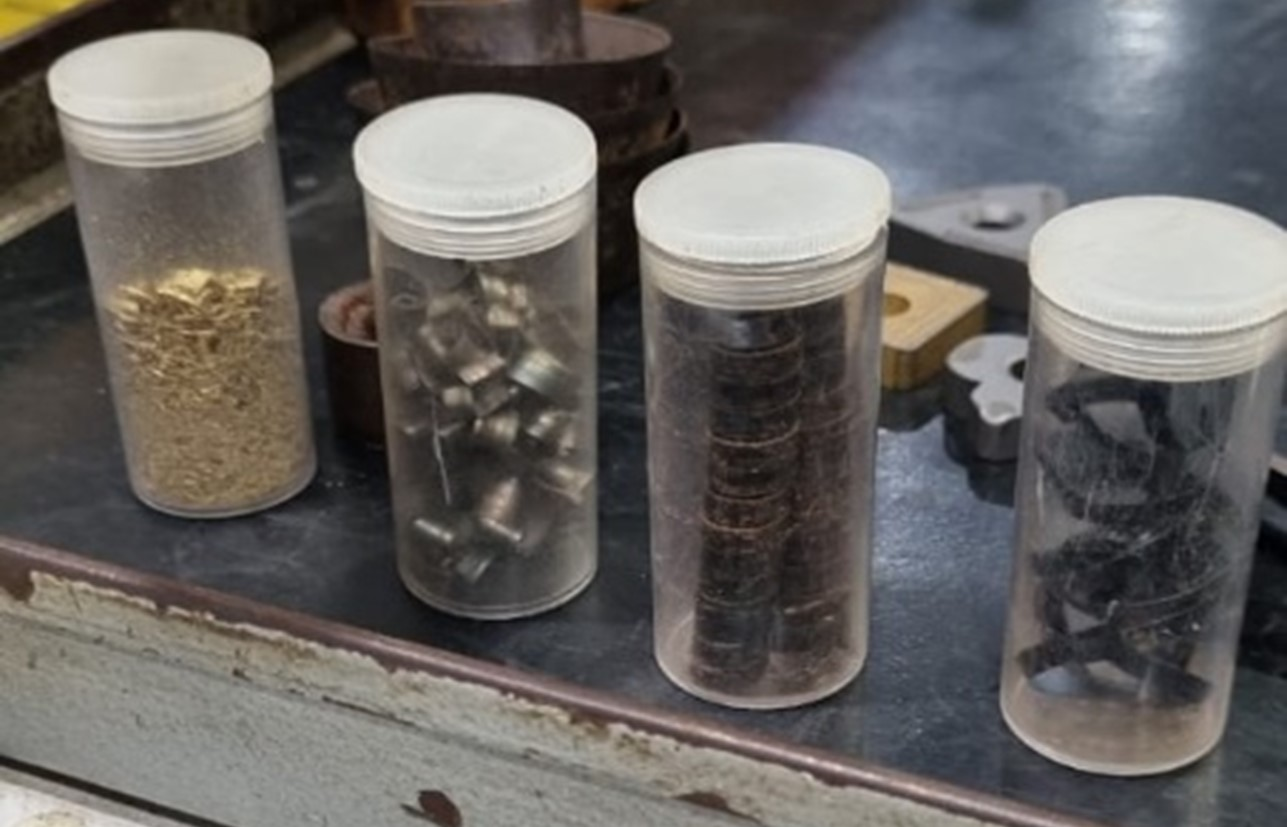
\includegraphics[width=1\linewidth]{Imagens/Exp03_cavacos.jpg}
    \smallcaption{Fonte: Autor}
    \label{fig:cavacos}
 \end{figure}
 
\subsection{Cavaco Fita / Espiral em Fita}

Os cavacos gerados possuem forma de segmentos contínuos, longos e afiados, frequentemente adotando um formato espiral. Esse tipo de cavaco é considerado ideal para operações de acabamento, sendo comumente observado em procedimentos de usinagem com baixa profundidade de corte. No entanto, seu formato também é seu maior risco, possuindo grande volume, apresentando perigo de corte quando manuseado inadequadamente, podendo ser observado no terceiro e quarto recipiente da Figura \ref{fig:cavacos}.

\subsection{Cavaco Cisalhado}

Os cavacos são descontínuos, cisalhados em pequenos pedaços quebradiços. Esse tipo de cavaco é considerado ideal para desbaste, sendo comumente observado em procedimentos de usinagem com alta avanço (facilitando a quebra). Mesmo sendo de fácil armazenamento, seu principal risco é seu formato e temperatura, devido a seu alta velocidade e avanço da máquina, este tipo de cavaco pode ser observado no segundo frasco da Figura \ref{fig:cavacos}.

\subsection{Cavaco de Ruptura}

Os cavacos apresentam como sua principal característica, serem descontínuos, similares a pequenas agulhas. Este tipo de cavaco não depende da geometria da ferramenta, do avanço e da rotação, dependendo exclusivamente dos elementos que compõem o material (latão, bronze, cobre, ferro fundido cinzento). Possui alto risco de perfuração, devido ao seu formato e tamanho, não sendo produzido no experimento, podendo ser observado no primeiro recipiente da Figura \ref{fig:cavacos}.

\section{Desgaste de Ferramenta}

Segundo,\textcite{amorim2002estudo}, existem num processo de usinagem duas causas fortes o suficiente para substituição de uma ferramento sendo elas Avarias/Falhas catastróficas (lascamentos ou tricas) e Desgaste excessivo (desgastes que altearão a condição de corte ou a qualidade), neste contexto é importante entender como se forma cada uma dessas situações e classificar-las.

\subsection{Desgaste de Flanco ou Frontal}

Notado por um rápido desgaste na parte frontal da ferramenta, resultando em um acabamento superficial inadequado ou fora das tolerâncias dimensionais desejadas, geralmente causado por altas velocidades de corte ou classe pouco resistente ao desgaste, Figura \ref{fig:flanco}. 

 \begin{figure}[!htb]
 \centering
    \caption{Representação esquemática desgaste de flanco}
    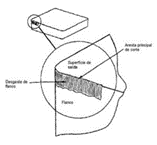
\includegraphics[width=0.3\linewidth]{Imagens/Exp03_Desgastedeflanco.png}
    \smallcaption{Fonte: \textcite{amorim2002estudo}}
    \label{fig:flanco}
 \end{figure}

\subsection{Desgaste de Cratera}

Caracterizado como uma “craterização” na superfície de saída, enfraquecendo a ferramenta e afetando o acabamento superficial, geralmente resultam de altas temperaturas e pressões exageradas sobre a superfície da ferramenta, sendo o tipo de desgaste que mais coloca em risco a peça, Figura \ref{fig:cratera}.

 \begin{figure}[!htb]
 \centering
    \caption{Representação esquemática desgaste de cratera}
    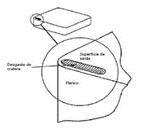
\includegraphics[width=0.3\linewidth]{Imagens/Exp03_Desgastedecratera.png}
    \smallcaption{Fonte: \textcite{amorim2002estudo}}
    \label{fig:cratera}
 \end{figure}

\subsection{Desgaste de tipo Entalhe}

Semelhante a uma trinca entre a superfície de saída e o flanco, esse tipo de desgaste pode resultar em um acabamento superficial de menor qualidade e levar a uma possível quebra da aresta, sendo frequentemente causado por altas velocidades de corte e pouca profundidade de corte, Figura \ref{fig:entalhe}.

 \begin{figure}[!htb]
 \centering
    \caption{Representação esquemática desgaste tipo entalhe}
    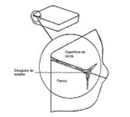
\includegraphics[width=0.3\linewidth]{Imagens/Exp03_Desgastetipoentalhe.png}
    \smallcaption{Fonte: \textcite{amorim2002estudo}}
    \label{fig:entalhe}
 \end{figure}

\subsection{Lascamento}

Ocorre um lascamento na zona de corte, levando a um acabamento superficial indesejado e um desgaste exagerado na parte frontal, causado por instabilidade no processo como um todo, pelo material e geometria da pastilha ou por fluido de corte insuficiente, Figura \ref{fig:lascamento}.

\begin{figure}[!htb]
 \centering
    \caption{Representação lascamento}
    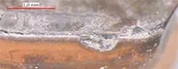
\includegraphics[width=0.4\linewidth]{Imagens/Exp03_Lascamento.png}
    \smallcaption{Fonte: \textcite{sandivik}}
    \label{fig:lascamento}
 \end{figure}

\subsection{Quebra de Arresta}

A quebra de aresta acontece principalmente em decorrer de uma possível pastilha desgastada, altas pressões de corte, classe da pastilha ser muito quebradiça, velocidade de corte irregular ou um avanço muito alto, Figura \ref{fig:quebra}.

\begin{figure}[!htb]
 \centering
    \caption{Representação quebra de aresta}
    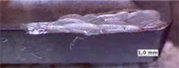
\includegraphics[width=0.4\linewidth]{Imagens/Exp03_quebra.png}
    \smallcaption{Fonte: \textcite{sandivik}}
    \label{fig:quebra}
 \end{figure}

\subsection{Quebra de Arresta}

As principais implicações da ocorrência de uma aresta postiça são um possível lascamento da aresta de corte e um acabamento superficial inadequado. Dessa forma, suas principais causas podem ser uma baixa temperatura na zona de corte, material pastoso e uma pastilha com geometria negativa, Figura \ref{fig:postiça}.

\begin{figure}[!htb]
 \centering
    \caption{Representação aresta postiça}
    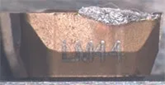
\includegraphics[width=0.4\linewidth]{Imagens/Exp03_postiça.png}
    \smallcaption{Fonte: \textcite{sandivik}}
    \label{fig:postiça}
 \end{figure}


\chapter{Metodologia}

Durante o processo experimental realizado em laboratório, foram realizados três procedimentos, com as seguintes especificações; Experimento 01: Tabela \ref{tab:exp1}, Experimento 02: Tabela \ref{tab:exp2} e Experimento 03: Tabela \ref{tab:exp3}.


\begin{table}[!htb]
 \centering
    \caption{Especificações experimento 1}
    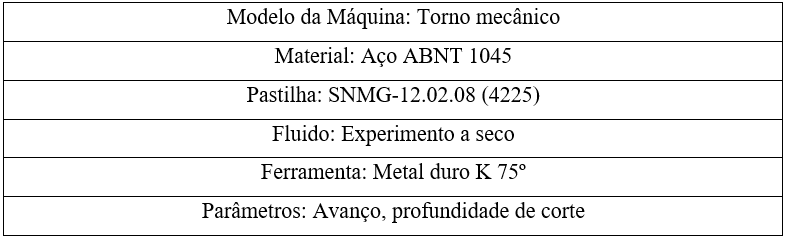
\includegraphics[width=0.65\linewidth]{Imagens/Exp03_exp1.png}
    \smallcaption{Fonte: Autor}
    \label{tab:exp1}
 \end{table}
 
\begin{table}[!htb]
 \centering
    \caption{Especificações experimento 3}
    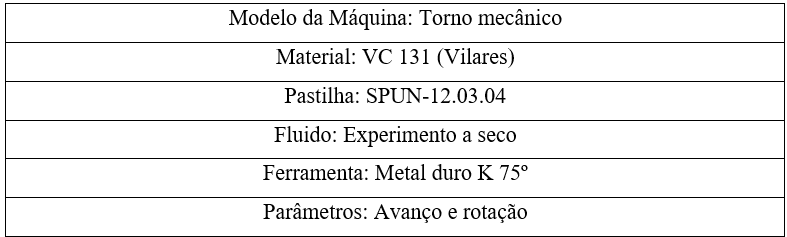
\includegraphics[width=0.65\linewidth]{Imagens/Exp03_exp2.png}
    \smallcaption{Fonte: Autor}
    \label{tab:exp2}
 \end{table}

 \begin{table}[!htb]
 \centering
    \caption{Especificações experimento 3}
    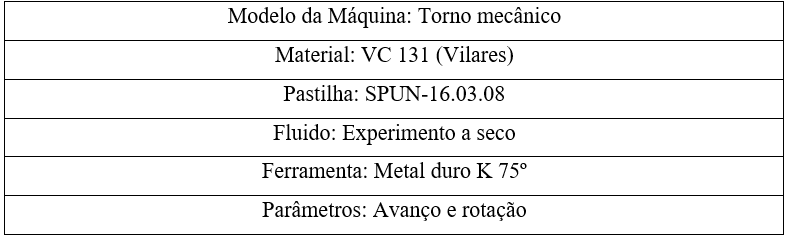
\includegraphics[width=0.65\linewidth]{Imagens/Exp03_exp3.png}
    \smallcaption{Fonte: Autor}
    \label{tab:exp3}
 \end{table}
 
\section{Experimento}

Inicialmente, a rotação foi fixada em 630 $RPM$ para o primeiro experimento, com uma profundidade de corte de 2 $mm$. Tendo isso em vista, o avanço foi sendo alterado através das alavancas da máquina, visando medir sua influência na espessura real do cavaco, que foi medida com um paquímetro convencional.

Já no segundo experimento, ocorreu a variação do avanço e rotação, utilizando a pastilha de metal duro K 75º. Nesse contexto, foi medido o tempo de usinagem com um cronômetro e o respectivo comprimento de usinagem com um paquímetro, além disso foi medida a temperatura do material e do cavaco.
 
Dando continuidade, foi caracterizado quais foram os tipos de cavaco obtidos, juntamente com os defeitos obtidos em cada ensaio, detalhados no referencial teórico. Ademais, todo o procedimento experimental do ensaio dois foi repetido para a ferramenta com ângulo de posição K90 (experimento 3), observando se ocorreu ou não desgaste em ambos os casos.

\begin{figure}[!htp]
  \centering
  \begin{minipage}{0.4\textwidth}
    \centering
    \caption{Torno Mecânico}
    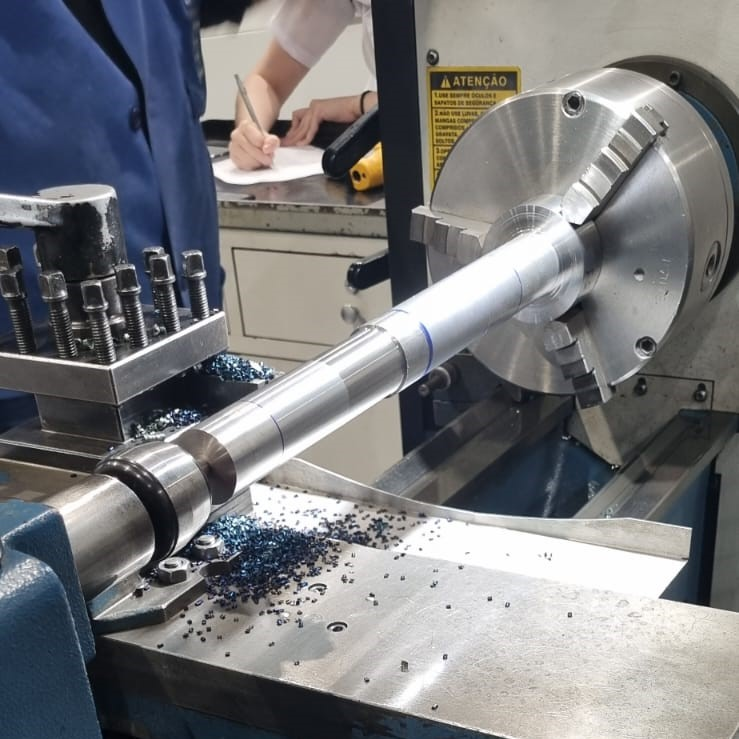
\includegraphics[width=1\linewidth]{Imagens/Exp03_torneamento.jpeg}
    \smallcaption{Fonte: Autor}
    \label{fig:CNC}
  \end{minipage}
  \hfill
  \begin{minipage}{0.4\textwidth}
        \caption{Ferramentas ultilizadas}
    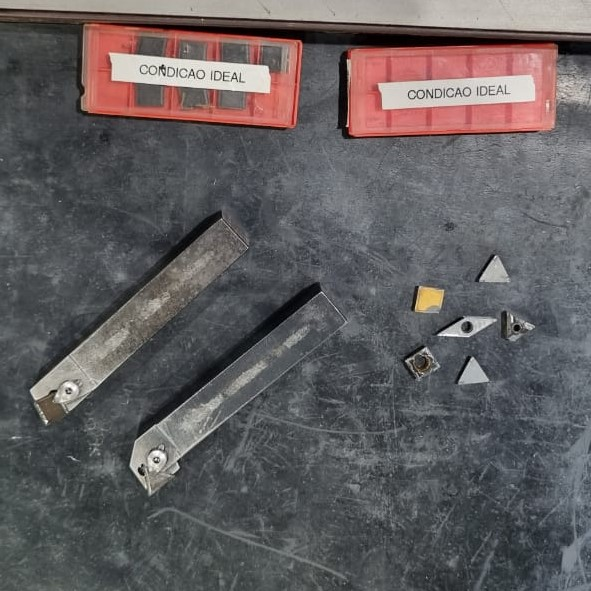
\includegraphics[width=1\linewidth]{Imagens/Exp03_ferramentas.jpeg}
    \smallcaption{Fonte: Autor}
    \label{fig:Ferramenta}
  \end{minipage}
\end{figure}

\chapter{Resultados e Discussões}

\section{Experimento 1}

 \begin{table}[!htb]
 \centering
    \caption{Cálculos e medições experimento 1}
    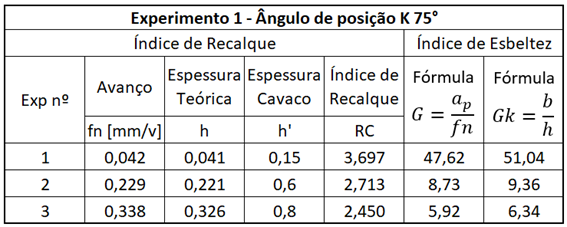
\includegraphics[width=0.8\linewidth]{Imagens/exp03_exp1dados.png}
    \smallcaption{Fonte: Autor}
    \label{tab:exp1dados}
 \end{table}

 Resultados superficiais: \\
1 – Cavaco espiral em fita com acabamento brilhoso\\
2 – Cavaco cisalhado com acabamento brilhoso\\
3 – Cavaco cisalhado com acabamento brilhoso\\

Após a medição da espessura real com uso do paquímetro, foi calculada a espessura teórica e o índice de recalque. Dessa forma, foi possível observar na Tabela \ref{tab:exp1dados} que o índice de recalque apresentou uma diminuição com o aumento do avanço ao longo dos ensaios, o que implica em um incremento no ângulo de cisalhamento, e na velocidade de saída do cavaco, gerando uma rugosidade menor e um melhor acabamento superficial. Vale ressaltar que, o índice de recalque e o ângulo de cisalhamento são possíveis indicadores da deformação presente no plano de cisalhamento primário \cite{hoffmann2020influencia}.  

Referente ao índice de esbeltez pode-se destacar que, os valores de G e Gk são próximos, e que foram diminuindo com o aumento do avanço nos ensaios. Diante disso, foi possível observar que a diminuição do índice de esbeltez levou a um aumento na rugosidade, tendo o Ensaio (1) com a melhor rugosidade \cite{dainfluencia}.

Ademais, pode-se acrescentar que, o acabamento superficial analisado está diretamente relacionado com a formação de cavaco, tendo uma melhor qualidade em cavacos contínuos pela menor força de corte presente no processo e uma qualidade inferior em cavacos de cisalhamento \cite{de2009analise}. 

\section{Experimento 2}

\begin{table}[!htb]
 \centering
    \caption{Cálculos e medições experimento 2}
    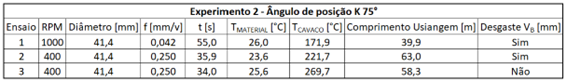
\includegraphics[width=1\linewidth]{Imagens/exp03_exp2dados.png}
    \smallcaption{Fonte: Autor}
    \label{tab:exp2dados}
 \end{table}
 
No primeiro ensaio a superfície obtida foi fosca, sem nenhum ruído, possuindo um cavaco cisalhado. Esse caso apresentou a menor temperatura do cavaco e o menor comprimento de usinagem, apresentando desgaste.

No segundo ensaio a ferramenta apresentou aresta postiça, levando a um acabamento superficial de menor qualidade. As possíveis causas para o ocorrido são a menor temperatura na zona de corte e a utilização de uma pastilha com geometria negativa. Ocorreu desgaste na ferramenta.

No terceiro ensaio foi obtida uma superfície com acabamento brilhoso, não ocorrendo desgaste neste caso, pois foi utilizada uma pastilha ideal para a peça. 

\section{Experimento 3}

 \begin{table}[!htb]
 \centering
    \caption{Cálculos e medições experimento 3}
    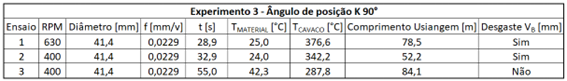
\includegraphics[width=1\linewidth]{Imagens/exp03_exp3dados.png}
    \smallcaption{Fonte: Autor}
    \label{tab:exp3dados}
 \end{table}
 
Sobre a ferramenta, a geometria desta também tem influência sobre a força de corte e o ângulo de saída da ferramenta é o mais influente, isto porque, quanto menor o ângulo de saída maior será a área de contato ferramenta-peça e, portanto, aumentará a força de corte, apresentando um acabamento superficial inferior à ferramenta de K75º

Os dois primeiros ensaios apresentaram aresta postiça, isso pode ter ocorrido pela geometria de corte ser muito negativa e pela temperatura desfavorável (muito alta). O que não ocorreu no terceiro ensaio, em que foi utilizada uma pastilha mais adequada para o caso estudado.


\chapter{Conclusões}

Em suma, ao longo do trabalho desenvolvido e das medições realizadas, foi possível entender a influência do avanço e profundidade de corte na formação de cavaco e no acabamento superficial, relacionando-os com os índices de recalque e esbeltez. Nesse ponto de vista, observou-se que para menores valores de avanço e, consequentemente, maiores valores de índice de recalque as superfícies apresentaram uma rugosidade menor e um melhor acabamento superficial.

Além disso, foi analisada a influência do uso da pastilha adequada e da mudança de ferramenta K75º para K90º, visando evitar o desgaste das ferramentas, no caso, aresta postiça e sua relação com as temperaturas do material e do cavaco.


\printbibliography

\end{document}